%%%%%%%%%%%%%%%%%%%%%%% file template.tex %%%%%%%%%%%%%%%%%%%%%%%%%
%
% This is a general template file for the LaTeX package SVJour3
% for Springer journals.          Springer Heidelberg 2010/09/16
%
% Copy it to a new file with a new name and use it as the basis
% for your article. Delete % signs as needed.
%
% This template includes a few options for different layouts and
% content for various journals. Please consult a previous issue of
% your journal as needed.
%
%%%%%%%%%%%%%%%%%%%%%%%%%%%%%%%%%%%%%%%%%%%%%%%%%%%%%%%%%%%%%%%%%%%
%
% First comes an example EPS file -- just ignore it and
% proceed on the \documentclass line
% your LaTeX will extract the file if required
\begin{filecontents*}{example.eps}
%!PS-Adobe-3.0 EPSF-3.0
%%BoundingBox: 19 19 221 221
%%CreationDate: Mon Sep 29 1997
%%Creator: programmed by hand (JK)
%%EndComments
gsave
newpath
  20 20 moveto
  20 220 lineto
  220 220 lineto
  220 20 lineto
closepath
2 setlinewidth
gsave
  .4 setgray fill
grestore
stroke
grestore
\end{filecontents*}
%
\RequirePackage{fix-cm}
%
%\documentclass{svjour3}                     % onecolumn (standard format)
%\documentclass[smallcondensed]{svjour3}     % onecolumn (ditto)
\documentclass[smallextended]{svjour3}       % onecolumn (second format)
%\documentclass[twocolumn]{svjour3}          % twocolumn
%
\smartqed  % flush right qed marks, e.g. at end of proof
%
%\usepackage{units}
%\usepackage{multirow}
%\usepackage{amstext}
%\usepackage{amsmath}
%\usepackage{amssymb}
%\usepackage{amsfonts}
\usepackage{enumerate}
\usepackage{cite}
%\usepackage{natbib}
%\usepackage{amsthm}
\usepackage{array,arydshln}
\usepackage[pdftex]{graphicx}
\usepackage{rotating}
\usepackage{ifpdf}
%\usepackage{epsfig}
\usepackage[all]{xy}
\usepackage{latexsym}
\usepackage[hidelinks]{hyperref}
\usepackage{color}
\usepackage{wrapfig}
\usepackage{caption}
%
\usepackage{mathptmx}      % use Times fonts if available on your TeX system
%
% insert here the call for the packages your document requires
%\usepackage{latexsym}
% etc.
%
% please place your own definitions here and don't use \def but
% \newcommand{}{}
%
% Insert the name of "your journal" with
% \journalname{myjournal}
%
\begin{document}

\title{Development of an Algorithm Improving Label Arrangements in Offset Printing}
%\subtitle{Do you have a subtitle?\\ If so, write it here}

%\titlerunning{Short form of title}        % if too long for running head

\author{Geun Soo Jang \and
        Taehyeong Kim \and\\
        Ki Man Kong \and
        Jeong Rye Park \and\\
        Jong-hyeon Seo \and
        Sang-hyup Seo$^\dagger$ \and\\
        Shin won Yoon
}

%\authorrunning{Short form of author list} % if too long for running head

\institute{Geun Soo Jang \at
              Finance.Fishery.Manufacture Industrial Mathematics Center on Big Data, Pusan National University, Busan, 46241, Republic of Korea \\
%              Tel.: +123-45-678910\\
%              Fax: +123-45-678910\\
              \email{sand621@naver.com}           %  \\
%             \emph{Present address:} of F. Author  %  if needed
           \and
           Taehyeong Kim \at
              Finance.Fishery.Manufacture Industrial Mathematics Center on Big Data, Pusan National University, Busan, 46241, Republic of Korea \\
              \email{xogud7936@pusan.ac.kr}           %  \\
           \and
           Ki Man Kong \at
           World Komax Co., Ltd., 1505, Centum Jungang-Ro 48,Haeundae-Gu, Busan, 48059, Republic of Korea \\
           \email{kennethkong@worldkomax.net}
           \and
           Jeong Rye Park \at
           Finance.Fishery.Manufacture Industrial Mathematics Center on Big Data, Pusan National University, Busan, 46241, Republic of Korea \\
           \email{parkjr@pusan.ac.kr}           %  \\
           \and
           Jong-hyeon Seo \at
           Chubu University Academy of Emerging Science, Kasugai, 487-0027, Japan \\
           \email{hyeonni94@gmail.com}
           \and
           Sang-hyup Seo \at
           $\dagger$Corresponding Author\\
           Finance.Fishery.Manufacture Industrial Mathematics Center on Big Data, Pusan National University, Busan, 46241, Republic of Korea \\
           \email{saibie1677@gmail.com}           %  \\
           \and
           Shin won Yoon \at
           Finance.Fishery.Manufacture Industrial Mathematics Center on Big Data, Pusan National University, Busan, 46241, Republic of Korea \\
           \email{ysw0123@pusan.ac.kr}
}

\date{Received: date / Accepted: date}
% The correct dates will be entered by the editor


\maketitle

%\thanks{}

\begin{abstract}
One of the most classic problems in the manufacturing industry is inventory processing. 
The best method to solve the problem is not to make any inventory. 
There is a way to effectively reduce inventory by merely changing the array of the pieces on the printing plates in the offset printing. 
It is setting an upper limit of acceptable for each plate and carrying out complete enumeration. 
These method reduce the accuracy, but dramatically reduces the operating time of the algorithm. 
The strength of this method lies in the fact that there is only change the arrangement of the pieces inside the plates.
%subject classification numbers as needed.
\keywords{Offset Printings \and Combinations with Repetition \and Label Arrangements \and Inventory Managements}
% \PACS{PACS code1 \and PACS code2 \and more}
% \subclass{MSC code1 \and MSC code2 \and more}
\end{abstract}

\section{Introduction}\label{sec:intro}
A combinations with repetition is the number of cases, where $k$ elements are selected from among different $n$ elements allowing repetition \cite{Brualdi2004}. 
It is indicated with the symbol $_{n}H_{k}$ and the following is established.
\begin{equation}
	_{n}H_{k} = _{n+k-1}C_{k} = \frac{(n+k-1)!}{(n-1)!k!}
\end{equation}
For instance, the combinations with repetition $_{2}H_{4}$ to select four elements from among two elements A and B comprises the following five cases.
\begin{enumerate}[(1)]
	\item $\textrm{[A, A, A, A]}$ : a list consisting of four A's
	\item $\textrm{[A, A, A, B]}$ : a list consisting of three A's and one B
	\item $\textrm{[A, A, B, B]}$ : a list consisting of two each of A's and B's
	\item $\textrm{[A, B, B, B]}$ : a list consisting of one A and three B's
	\item $\textrm{[B, B, B, B]}$ : a list consisting of four B's
\end{enumerate}
Among the above cases, if we want to obtain three A's and nine B's, then we can choose $[\textrm{A, B, B, B}] \times 3$. 
Let us consider the following.
\begin{equation}
	\textrm{[A, A, B, B]} \times 1 + \textrm{[A, B, B, B]} \times 1 + \textrm{[B, B, B, B]} \times 1
\end{equation}
In this case, we can get the three A's and nine B's. 
However, the former case seems to be a ‘Better’ because making three different lists is inefficient. 
Let us examine another case.
\begin{equation}
\textrm{[A, A, A, A]} \times 1 + \textrm{[B, B, B, B]} \times 3 - \textrm{[A]} \times 1 - \textrm{[B]} \times 3
\end{equation}
$\textrm{[A, B, B, B]} \times 3$ also seems to be 'Better' because there is no loss. Under the following conditions, $\textrm{[A, B, B, B]} \times 3$ is the ‘Best’ method.
\begin{enumerate}[(1)]
	\item Minimize the number of list.
	\item Minimize the loss of lists.
\end{enumerate}
Offset printing, also called offset lithography, or litho-offset, in commercial printing, 
widely used printing technique in which the inked image on a printing plate is printed on a rubber cylinder and then transferred (i.e., offset) to paper or other material. 
The rubber cylinder gives great flexibility, permitting printing on wood, cloth, metal, leather, and rough paper (see Figure \ref{fig:OffsetPrint}) \cite{OffsetPrint}.

\begin{figure}[h!]
	\centering
	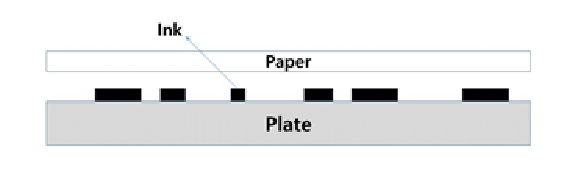
\includegraphics[width=7cm]{OffsetPrint.pdf}
	\caption{Offset Printing}
	\label{fig:OffsetPrint}
\end{figure}

Offset lithography is one of the most common ways of creating printed materials. A few of its common applications include: newspapers, magazines, brochures, stationery, and books. Compared to other printing methods, offset printing is best suited for economically producing large volumes of high quality prints in a manner that requires little maintenance \cite{Kipphan2001}. Therefore, how to make the initial plates is an important issue. Above example means that what is the best arrangement in such print method.

In the past, production was based on ordering of products from companies. For instance, apparel companies stocked popular products in warehouses. If the companies didn't have inventory, then consumers could not obtain rare sized or unpopular products. However, as the Internet market has became popular, the production systems have been changed into systems. Factories do not produce products based on their prediction of consumption but do produce only ordered products.

World Komax is a company that produces labels using the offset printing. The labels refer to stickers containing bar-codes attached to garments or shoes as follows (see Figure \ref{fig:AirHuarache}). Each bar-code in the label contains fixed information such as product names and colors, and variable information such as the date of manufacture.

\begin{figure}[h!]
	\centering
	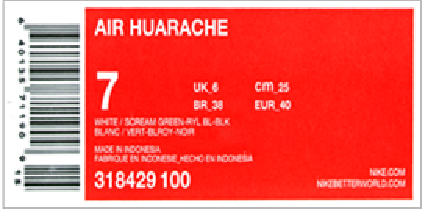
\includegraphics[width=6.5cm]{AirHuarache.pdf}
	\caption{Sneaker Review : Nike Air Huarache (http://visla.kr/?p=18146)}
	\label{fig:AirHuarache}       % Give a unique label
\end{figure}

Since the program of World Komax is not suitable for small quantity batch productions, the number of labels loss increased compared to the past.

Section 2 of this paper will describe the process of label printing using offsets. The modeling of the problem will be carried out in Section 3, and examples to help the understanding of the problem will be prepared in Section 4. The final results of the algorithm will be described in Section 5. 


\section{Offset label printing process}\label{sec:Offset}

\subsection{Label printing process}\label{subsec:LabelPrinting}
Prior to describing the label printing process, we define the following terms first.
\begin{enumerate}[*]
	\item {\bf Plate} : A printing plate for the offset printing (see Figure \ref{fig:PlateLabel})
	\item {\bf Loss} : The number of labels printed in excess of the order-quantity
\end{enumerate}

\begin{wrapfigure}{r}{4cm}
	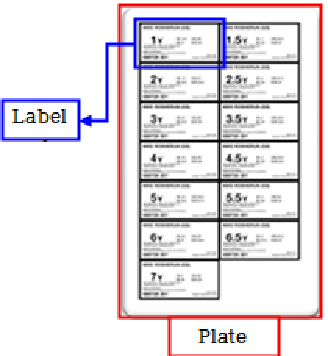
\includegraphics[width=4cm]{PlateLabel.pdf}
	\caption{Plate and Label}
	\label{fig:PlateLabel}       % Give a unique label
\end{wrapfigure}

The offset label printing process is as follows. At first, we receive orders from customers. The order includes many types of labels to be printed and order-quantities by type (see Figure \ref{fig:Order_Sorting}). Thereafter, offset printing plates are made. Many types of labels are placed on each plate so that many labels are printed at one printing. When the plates have been made, the printing operation is carried out so that individual labels are produced in quantities not smaller than the order-quantities using individual plates. As the final process, the sheets are cut to the sizes of labels and labels are collected by type.

\subsection{Major points for cost saving}\label{subsec:CostSave}
The constraint conditions and major points that will be considered in this paper for cost saving are as follows. First, one type of label should be placed on only one plate. This is to prevent different types of labels from being mixed when collected by type after the printed sheets are cut. Meanwhile, the total number of labels placed on each plate is also constant because the sizes of individual plates are constant and the sizes of labels in one order are also constant. In addition, the number of plates should be minimized as little as possible because plates are made using molds and the costs are high. Finally, the losses of labels printed should be minimized because bar-codes which are used only one time are printed in the labels and if the inventory remains, they cannot be used and should be entirely discarded.

\subsection{Sorting report output program}\label{subsec:SortProgram}
Plate fabrication and the use of printing paper incur costs. In order to reduce the costs, order details are inputted to output appropriate methods to place labels on the plate as sorting reports. The plate makers produce plates according to the instructions in the sorting reports (see Figure \ref{fig:Order_Sorting}).

Since the existing sorting report output method was not suitable for small quantity batch production systems, the algorithm should be improved. Therefore, this study was conducted to develop new algorithms suitable for small quantity batch production systems too.

\begin{figure}[h!]
	\centering
	\resizebox{11cm}{4cm}{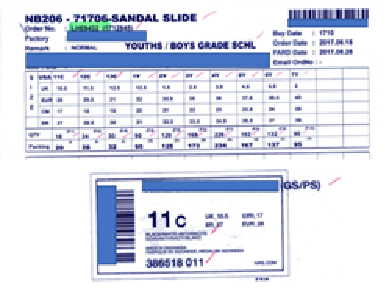
\includegraphics{OrderForm.pdf}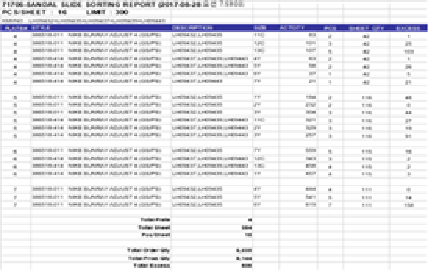
\includegraphics{SortingReport.pdf}}
	\caption{An Order Form(left) and a Sorting Report(right) \\(Source: World Komax Co., Ltd.)}
	\label{fig:Order_Sorting}       % Give a unique label
\end{figure}

\section{Modeling and flowchart}\label{sec:Modeling}
To accurately formulate our problem as a mathematical optimization problem, we first need to define our notation.
\begin{enumerate}[$\bullet$]
	\item Let $I$ be a set of products.
	\item For each product $i \in I$, let $b_{i}$ be the number of order.
	\item Let ${\bf b}=(b_{i}|i \in I)$ be a vector of order-quantities.
	\item $k$ is the total number of labels that can be placed in one Plate.
	\item $\pi$ is a partition of $I$ such that $1 \leq  |P| \leq k$ for any $P \in \pi$. 
	\item Let $\Gamma_{\pi}$ be a set of matrix $A \in {\rm Mat}_{\pi \times I}(\mathbf{Z})$ satisfy the following:
	\begin{description}[-]
		\item For all $(P,i) \in \pi \times I$, $A_{P,i} \geq 0$, and $A_{P,i} = 0$ if and only if $i \notin P$.
		\item For each $P \in \pi$, $\sum_{i \in P}A_{P, i} = k$
\end{description}
\end{enumerate}

Using the above notation,
\begin{equation}\label{eq:NumPlate}
	\left\lceil \max \left\{ \left.\frac{b_{i}}{A_{P,i}}\right|i \in P \right\} \right\rceil
\end{equation}
is the number of printing of Plate $P$, where $\lceil~\rceil$ means the ceiling. 
Assume that $\alpha$ is the cost to produce one Plate, and $\beta$ is the cost of the loss of one label. 
Then, our goals is to obtain the following 
\begin{equation}\label{eq:TotalCost}
	\min_{\pi} \{ \alpha|\pi| + \beta E_{A,b} | A \in \Gamma_{\pi} \}
\end{equation}
where
\begin{equation}\label{eq:TotalLoss}
	E_{A,b} = \sum_{P \in \pi} \sum_{i \in I} \left( \left\lceil \max \left\{ \left.\frac{b_{i}}{A_{P,i}}\right|i \in P \right\} \right\rceil \cdot A_{P,i} - b_{i} \right)
\end{equation}
means the total number of losses of labels.

Naturally, the complete enumeration using combinations with repetition is the surest way. 
However, this method has a problem of taking too much time. 
For instance, when $n=65$ and $k = 24$, the combination with repetition $_{65}H_{24}$ comprises $2.36 \times 10^{21}$ cases, 
and the calculation of the cases takes more than 658 hours, that is, more than 27 days using a super computer that can calculate $10^{15}$ partitions per second. 
Given that there are limits of the time from the date of receipt of orders to the delivery date, this is a very long computation time.

In this algorithm, this problem was solved by introducing any positive integers as tolerances. 
Tolerances means the allowed amount of losses occurring in each plate. 
Adopting a partition that does not exceed the tolerance will dramatically reduce the time taken.

\begin{figure}[h!]
	\centering
	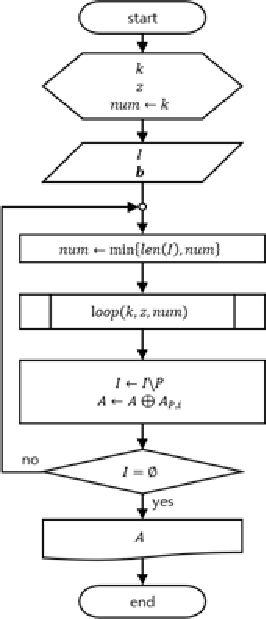
\includegraphics[width=3cm]{MainFChart.pdf}
	\caption{The Main Flow Chart}
	\label{fig:MFChart}       % Give a unique label
\end{figure}

Based on the foregoing, the flowchart of the algorithm can be set forth as follows. 
This algorithm outputs matrix $A$ containing the label of each product when $I$ and ${\bf b}$ have been inputted for $z$, $k$, $num$ (see Figure \ref{fig:MFChart}). 

\begin{figure}[h!]
	\centering
	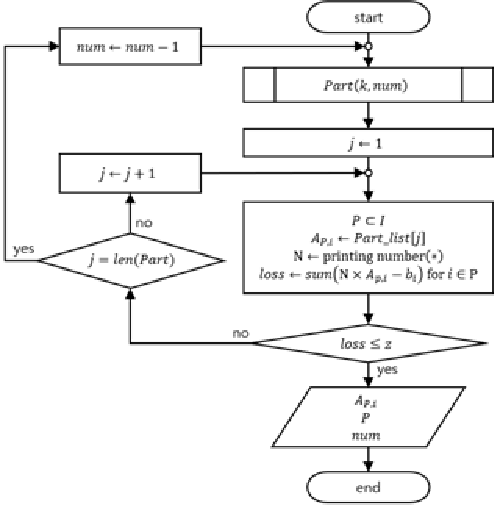
\includegraphics[width=5cm]{SubFChart.pdf}
	\caption{The Flow Chart of Loop}
	\label{fig:SFChart}       % Give a unique label
\end{figure}

Meanwhile, in the case of the ${loop}(k, z, num)$ function, the following flowchart should be followed.
First, the ${Part}(k, num)$ function finds partitions using the combination with repetition $_{num}H_{k}$ 
(method to select $k$ pieces of products from $num$ pieces of products allowing repetition) and indicated in the form of a list. 
We set the result as {\it Part\underline{ }list}. 
An appropriate $P$ that has $num$ pieces of products is selected from $I$ and the loss is obtained using {\it Part\underline{ }list} and the printing number.

If the loss exceeds the tolerance $z$, another {\it Part\underline{ }list} will be selected and the foregoing will be repeated 
while adjusting $num$ until the tolerance is not exceeded.
As a result of this process, $A_{P,i}$ that does not exceed the tolerance is obtained (see Figure \ref{fig:SFChart}).



\section{Examples}\label{sec:Exam}
This example was described to help the understanding of the problem. In this section, we assume that $k$ is equal to 4.

\begin{example}
	Let $I=\{A,B,C\}$ and ${\bf b}=(50,30,20)$.
	
	We consider $\pi = \{\{A, B\}, \{C\}\}$ is a partition for the order-quantity vector ${\bf b}$. 
	Without loss of generality, assume that $P_{1} = \{A, B\}, P_{2} = \{C\}$. Since $k = 4$, the matrix $A$ can be found as follows.
	
	\begin{equation}
		A = \left(\begin{array}{ccc}2 & 2 & 0 \\ 0 & 0 & 4 \end{array}\right)
	\end{equation}
	
	In this case, the printing numbers (\ref{eq:NumPlate}) of $P_1$ and $P_2$ are as follows, respectively.
	\begin{equation}
		\left\lceil \max\left\{ \left. \frac{b_{i}}{A_{P_{1},i}} \right| i \in P_{1} \right\} \right\rceil = \left\lceil \max \left\{ \frac{50}{2}, \frac{30}{2} \right\} \right\rceil = 25
	\end{equation}
	and
	\begin{equation}
	\left\lceil \max\left\{ \left. \frac{b_{i}}{A_{P_{2},i}} \right| i \in P_{2} \right\} \right\rceil = \left\lceil \max \left\{ \frac{20}{4} \right\} \right\rceil = 5.
	\end{equation}
	We can see the Figure \ref{fig:ex11} for more details.
	
	\begin{figure}[h!]
		\centering
		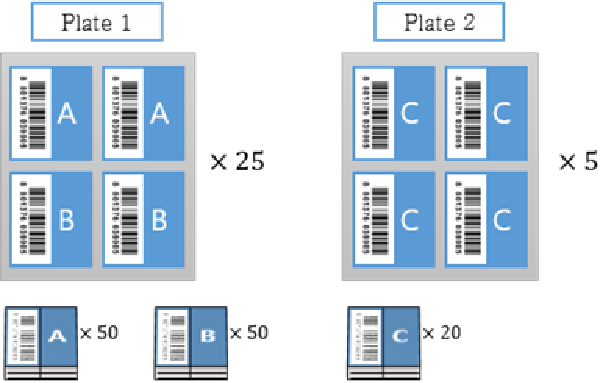
\includegraphics[width=6cm]{ex11.pdf}
		\caption{}
		\label{fig:ex11}       % Give a unique label
	\end{figure}
	
	It can be seen that the total number of Loss $E_{A,{\bf b}}$ is 20.
	
	Now, we consider a new partition $\pi = \{\{A, B, C\}\}$. In this case, $A = (\begin{array}{ccc}2 & 1 & 1 \end{array})$, and printing number (\ref{eq:NumPlate}) is 
	\begin{equation}
	\left\lceil \max\left\{ \left. \frac{b_{i}}{A_{P,i}} \right| i \in P \right\} \right\rceil = \left\lceil \max \left\{ \frac{50}{2}, \frac{30}{1}, \frac{20}{1} \right\} \right\rceil = 30.
	\end{equation}
	In addition, it can be easily seen that the total number of Loss $E_{A,{\bf b}}$ is 20 (see Figure \ref{fig:ex12}).
	Figure \ref{fig:ex12} is a more efficient because its Loss is the same but its number of Plates is smaller.
	\begin{figure}[h!]
		\centering
		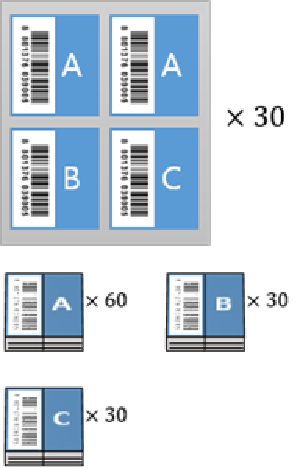
\includegraphics[width=3cm]{ex12.pdf}
		\caption{}
		\label{fig:ex12}       % Give a unique label
	\end{figure}
\end{example}

\begin{example}
	Assume that $I=\{A,B\}$, and the order-quantity vector ${\bf b}=(50,20)$.
	
	We consider $\pi = \{\{A,B\}\}$ is a partition for the quantity vector ${\bf b}$. Since $k = 4$, 
	the matrix $A = (\begin{array}{cc}2 & 2\end{array})$, and the printing number (\ref{eq:NumPlate}) is 
	\begin{equation}
	\left\lceil \max\left\{ \left. \frac{b_{i}}{A_{P,i}} \right| i \in P \right\} \right\rceil = \left\lceil \max \left\{ \frac{50}{2}, \frac{20}{2} \right\} \right\rceil = 25.
	\end{equation}
	The total number of Loss $E_{A,{\bf b}}$ is 30 (see Figure \ref{fig:ex21}).
	
	\begin{figure}[h!]
		\centering
		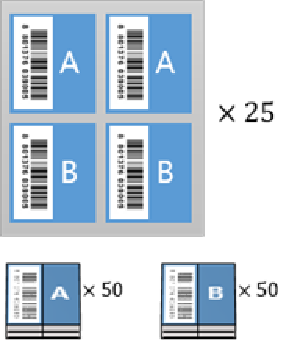
\includegraphics[width=3cm]{ex21.pdf}
		\caption{}
		\label{fig:ex21}       % Give a unique label
	\end{figure}
	
	For the same partition $\pi$, the matrix $A = (\begin{array}{cc}3 & 1\end{array})$ can be considered. In this case, the printing number (\ref{eq:NumPlate}) is 
	\begin{equation}
	\left\lceil \max\left\{ \left. \frac{b_{i}}{A_{P,i}} \right| i \in P \right\} \right\rceil = \left\lceil \max \left\{ \frac{50}{3}, \frac{20}{1} \right\} \right\rceil = 20.
	\end{equation}
	and the total number of Loss $E_{A,{\bf b}}$ is 10 (see Figure \ref{fig:ex22}).
	Figure \ref{fig:ex22} is more efficient because its number of Plate is the same but fewer losses occur.
	\begin{figure}[h!]
		\centering
		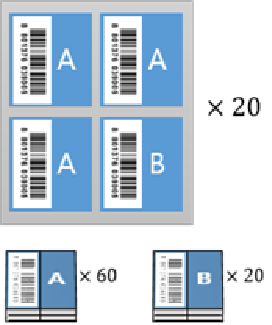
\includegraphics[width=3cm]{ex22.pdf}
		\caption{}
		\label{fig:ex22}       % Give a unique label
	\end{figure}
\end{example}

\section{Result}\label{sec:Result}

Each sorting report indicates the number of losses corresponding to one plate. 
Using this, the total cost can be obtained by replacing all plates with losses. 
We used 30 sorting report samples and it could be seen that the total cost decreased further 
when the algorithm in this study was applied than when the algorithm of the manufacturer was applied for all samples. 
It was identified that when the improved algorithm was used, the total cost was reduced by from minimum 0.4\%(sample no. 15) to maximum 15.96\%(sample no. 8) (see Figure \ref{fig:Comparing}).

\begin{figure}[h!]
	\centering
	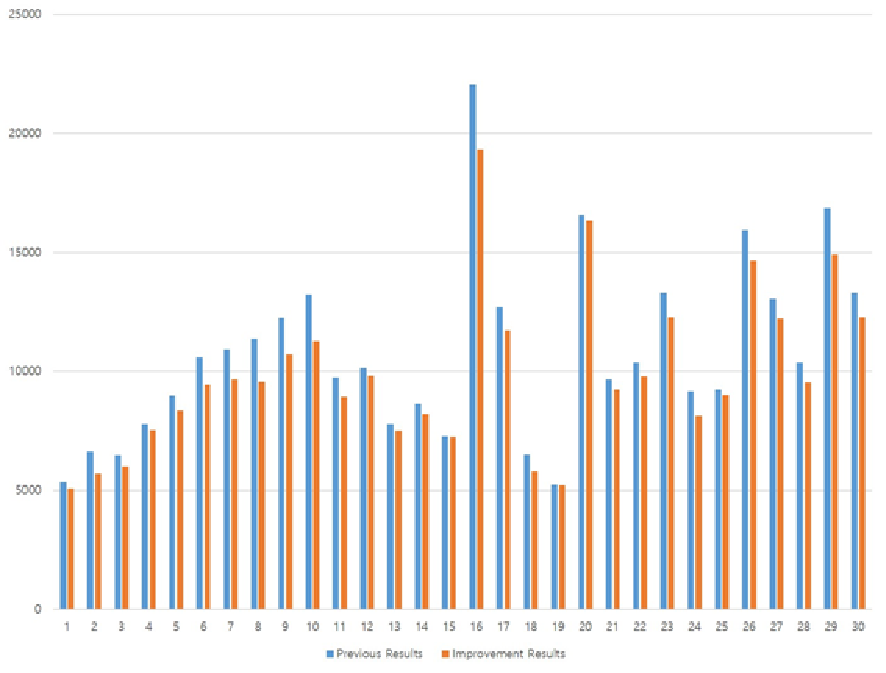
\includegraphics[width=\linewidth]{Comparing.pdf}
	\caption{Comparing the Results}
	\label{fig:Comparing}       % Give a unique label
\end{figure}

We used a paired t-test to verify the efficiency of the algorithm. The pared t-test is two sample t-test, and it is a test that verifies whether the two groups are different. The data were provided by the aforementioned company, and the two populations are as follows.

\begin{enumerate}[$\bullet$]
	\item population1: total cost before applying the algorithm
	\item population2: total cost after applying the algorithm
	\item sample1: sample of 30 items from population1
	\item sample2: sample of 30 items from population2
\end{enumerate}

In order to proceed with the two-sample t-test, the two groups must first satisfy the normality and homoscedasticity. The number of samples extracted from the two populations is 30, which can be said to have normality based on the central limit theorem. In addition, we identified the homoscedasticity of the two samples through the var.test of R.

The null hypothesis $(H_{0})$ of var.test is that 'the variances of the two groups are equal', and the alternative hypothesis$(H_{1})$ is that 'the variances of the two groups are different'. 
If the p-value is below the significance level, the null hypothesis $(H_{0})$ will be rejected and if the p-value is not lower than the significance level, the alternative hypothesis $(H_{1})$ will be rejected.  The result of var.test with the significance level to 0.05 is as follows.

\begin{figure}[h!]
	\centering
	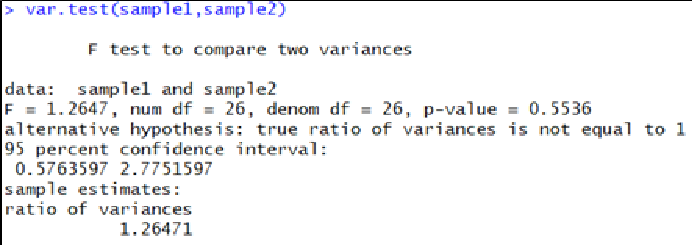
\includegraphics[width=9cm]{vartest.pdf}
	\caption{var.test of R}
	\label{fig:vartest}       % Give a unique label
\end{figure}

Since the p-value is not lower than the significance level(0.05), the alternative hypothesis $(H_{1})$ is rejected and the null hypothesis $(H_{0})$ is adopted. 
That is, the variances of the two groups can be said to be equal.

Since the two groups satisfy normality and homoscedasticity, we verified whether the difference between the two groups is significant through paired t-test. In this test, the null hypothesis $(H_{0})$ is ‘the total cost will be the same after applying the algorithm.’ and the alternative hypothesis $(H_{1})$ is ‘the total cost will be reduced after applying algorithm.’ The result of the paired t-test with the significance level to 0.05 is as follows.

\begin{figure}[h!]
	\centering
	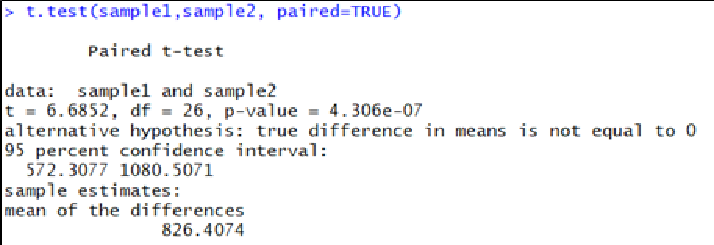
\includegraphics[width=9cm]{ttest.pdf}
	\caption{t.test of R}
	\label{fig:ttest}       % Give a unique label
\end{figure}

Since the p-value is below the significance level(0.05), the null hypothesis $(H_{0})$ is rejected and the alternative hypothesis $(H_{1})$ is adopted. That is, the difference between the two groups can be said to be significant.

{\bf Notice.} Please note that the detailed idea of the algorithm cannot be described for confidentiality of the company.

%\paragraph{Paragraph headings} Use paragraph headings as needed.
% For one-column wide figures use
%\begin{figure}
%% Use the relevant command to insert your figure file.
%% For example, with the graphicx package use
%  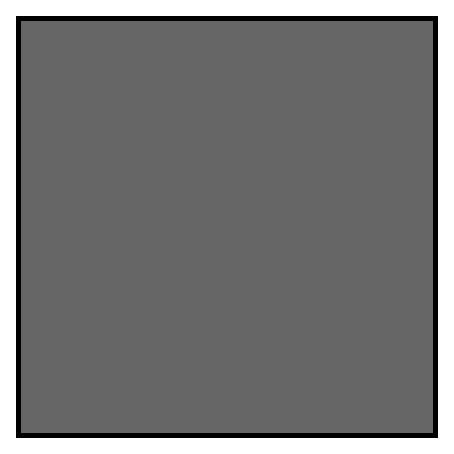
\includegraphics{example.eps}
%% figure caption is below the figure
%\caption{Please write your figure caption here}
%\label{fig:1}       % Give a unique label
%\end{figure}
%%
%% For two-column wide figures use
%\begin{figure*}
%% Use the relevant command to insert your figure file.
%% For example, with the graphicx package use
%  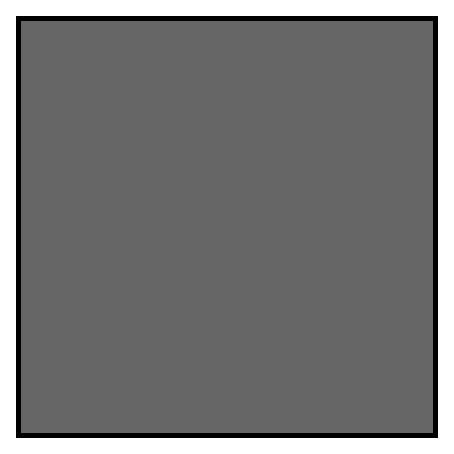
\includegraphics[width=0.75\textwidth]{example.eps}
%% figure caption is below the figure
%\caption{Please write your figure caption here}
%\label{fig:2}       % Give a unique label
%\end{figure*}
%
% For tables use
%\begin{table}
%% table caption is above the table
%\caption{Please write your table caption here}
%\label{tab:1}       % Give a unique label
%% For LaTeX tables use
%\begin{tabular}{lll}
%\hline\noalign{\smallskip}
%first & second & third  \\
%\noalign{\smallskip}\hline\noalign{\smallskip}
%number & number & number \\
%number & number & number \\
%\noalign{\smallskip}\hline
%\end{tabular}
%\end{table}


\begin{acknowledgements}
This work was supported by the National Research Foundation of Korea (NRF)
grant funded by the Korean Government (MSIP) (NRF-2017R1A5A1015722, NRF-2018R1D1A1B07048197). 
%The authors thank the anonymous referees for providing very useful suggestions for improving this paper.
The authors extend thanks to Professor Hyun-Min Kim and Professor Sang-il Kim of Pusan National University who provided many support and advises for the writing of this paper.
\end{acknowledgements}

% BibTeX users please use one of
%\bibliographystyle{spbasic}      % basic style, author-year citations
%\bibliographystyle{spmpsci}      % mathematics and physical sciences
%\bibliographystyle{spphys}       % APS-like style for physics
%\bibliography{}   % name your BibTeX data base

% Non-BibTeX users please use
\begin{thebibliography}{}
%
% and use \bibitem to create references. Consult the Instructions
% for authors for reference list style.
%
%\bibitem{RefJ}
%% Format for Journal Reference
%Author, Article title, Journal, Volume, page numbers (year)
%% Format for books
%\bibitem{RefB}
%Author, Book title, page numbers. Publisher, place (year)
% etc
\bibitem{Brualdi2004}
R. A. Brualdi, Introductory Combinatorics, Pearson Prentice Hall (2004)
\bibitem{Kipphan2001}
H. Kipphan, Handbook of Print Media: Technologies and Production Methods, Springer (2001)
\bibitem{OffsetPrint}
``Offset printing'', Encyclop{\ae}dia Britannica, inc., 19-06-2016.\\ url: https://www.britannica.com/technology/offset-printing.

\end{thebibliography}

\end{document}
% end of file template.tex

